%-------------------------------------------------
%
% Generator.tex
%
%------------------------------------------------
\section[Generatori di dati]{generatori di dati}
\label{pt1:generator}
Al fine di ottenere una discreta quantità di dati su cui effettuare dei test si è progettato e conseguentemente implemento, in linguaggio $C++$,
una serie di generatori di istanze.

I generatori creati sono in grado di:

\begin{itemize}
\item generare punti random su di una superficie di dimensioni date
\item generare punti riuniti in cluster su di una superficie di dimensioni date
\item generare punti su di una circonferenza di raggio e centro arbitrari all'interno di una superficie di dimensioni date.
\end{itemize}

In Figura \ref{pt1:generator:imgs} sono riportati alcuni esempi di dati generati attraverso le varie tipologie di generatori

\begin{figure}
\centering
\begin{subfigure}[h]{0.45\textwidth}
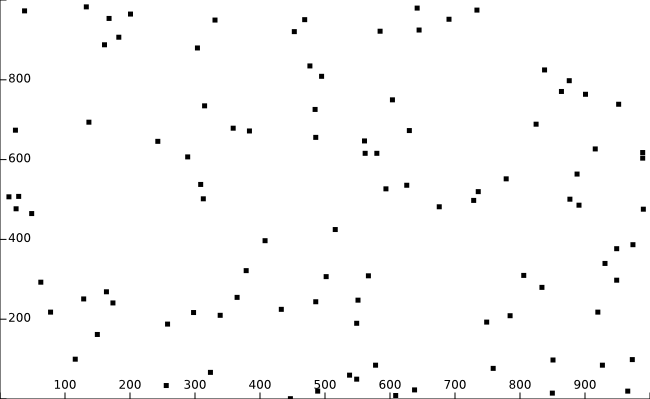
\includegraphics[width=\textwidth]{Images/Part_1/Instances/Random.png}
\caption{Random}
\label{pt1:generator:random_img}
\end{subfigure}
\quad{}
\begin{subfigure}[h]{0.45\textwidth}
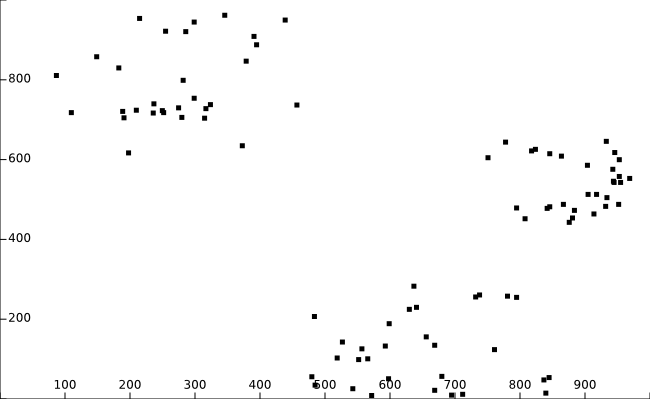
\includegraphics[width=\textwidth]{Images/Part_1/Instances/Cluster.png}
\caption{Cluster}
\label{pt1:generator:cluster_img}
\end{subfigure}

\begin{subfigure}[h]{0.5\textwidth}
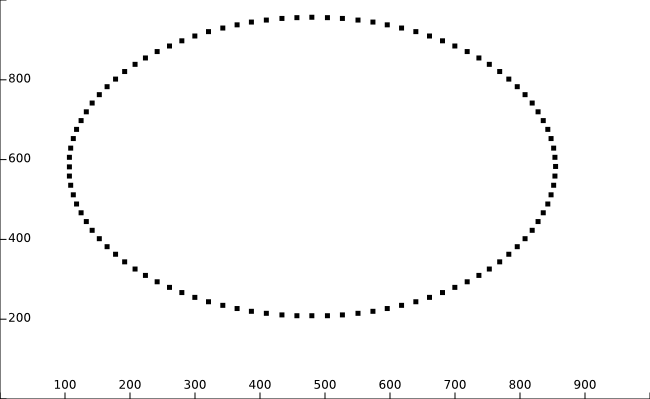
\includegraphics[width=\textwidth]{Images/Part_1/Instances/Circle.png}
\caption{Circonferenza}
\label{pt1:generator:Circle_img}
\end{subfigure}
\caption{Esempi di istanze generate}
\label{pt1:generator:imgs}
\end{figure}